% This LaTeX was auto-generated from MATLAB code.
% To make changes, update the MATLAB code and export to LaTeX again.

\documentclass{article}

\usepackage[utf8]{inputenc}
\usepackage[T1]{fontenc}
\usepackage{lmodern}
\usepackage{graphicx}
\usepackage{color}
\usepackage{hyperref}
\usepackage{amsmath}
\usepackage{amsfonts}
\usepackage{epstopdf}
\usepackage[table]{xcolor}
\usepackage{matlab}

\sloppy
\epstopdfsetup{outdir=./}
\graphicspath{ {./parte2_images/} }

\begin{document}

\matlabtitle{II. Equilibrio general}

\begin{par}
\begin{flushleft}
Ahora resolveremos el problema del pescador endogenizando los precios de la economía. Para ello asumiremos que la productividad marginal del trabajo está dada por
\end{flushleft}
\end{par}

\begin{par}
$$\omega =\frac{\partial }{\partial L}F\left(K,L\right)=\left(1-\alpha \right)\;{\left\lbrack \frac{K}{\bar{\;L} }\right\rbrack }^{\alpha }$$
\end{par}

\matlabheading{f. Demuestre que la demanda por capital K y el salario $\omega$ están dados por:}

\begin{par}
$$\begin{array}{l}
K={\left(\frac{\alpha }{r+\delta }\right)}^{\frac{1}{1-\alpha }} \cdot \bar{L} \;\;\;\;\;\;\;\;\;\;\;\;\;\;\;\;\;\;\;\;\;\;\;\;\;\;\;\;\;\;\;\;\;\;\;\;\left(1\right)\\
\omega =\left(1-\alpha \right){\left(\frac{\alpha }{r+\delta }\right)}^{\frac{\alpha }{1-\alpha }} \;\;\;\;\;\;\;\;\;\;\;\;\;\;\;\;\;\;\;\;\;\;\;\;\;\;\;\;\;\left(2\right)
\end{array}$$
\end{par}

\begin{par}
\begin{flushleft}
Primero, debemos partir encontrando las condiciones de primer orden de la función de beneficio. 
\end{flushleft}
\end{par}

\begin{par}
$$\begin{array}{l}
\textrm{Sabemos}\;\textrm{que}\;\textrm{la}\;\textrm{función}\;\textrm{de}\;\textrm{producción}\;\textrm{es}\;\;F\left(K,L\right)=K^{{\;}^{\alpha } } L^{{\;}^{1-\alpha } } ,p\;\textrm{el}\;\textrm{precio}\;\textrm{del}\;\textrm{bien}\;\textrm{que}\;\textrm{las}\;\textrm{empresas}\;\textrm{venden},L\;\textrm{el}\;\textrm{empleo},w\;\textrm{el}\;\textrm{salario},K\;\textrm{el}\;\textrm{capital}\;y\;R=\left(r+\delta \right)\;\textrm{su}\;\textrm{costo}\;\textrm{de}\;\textrm{uso}\\
\\
\;\;\;\;\;\;\;\;\;\;\;\;\;\;\;\;\;\;\;\;\;\;\;\;\;\;\;\;\;\;\;\;\;\;\;\;\;\;\;\;\;\;\;\;\;\;\;\;\;\;\;\;\;\;\;\;\;\;\Pi \left(p,w,r,\delta \right)=\max_{K,L} \;\;p\cdot \;F\left(K,L\right)-\left(\omega \cdot L+\left(r+\delta \right)K\right)
\end{array}$$
\end{par}

\begin{par}
$$\begin{array}{l}
{\textrm{PMG}}_k \equiv \frac{\partial }{\partial K}\Pi =\alpha \;{\left(\frac{L}{K}\right)}^{1-\alpha } -\left(r+\delta \right)=0\\
{\textrm{PMG}}_L \equiv \frac{\partial }{\partial L}\Pi =\left(1-\alpha \right)\cdot {\left(\frac{K}{L}\right)}^{\alpha } -\omega =0
\end{array}$$
\end{par}

\begin{par}
\begin{flushleft}
Despejando ${\textrm{PMG}}_k$ obtenemos que
\end{flushleft}
\end{par}

\begin{par}
$$\begin{array}{l}
\alpha \;{\left(\frac{L}{K^* }\right)}^{1-\alpha } =\;\left(r+\delta \right)\leftrightarrow {\left(K^* \right)}^{1-\alpha } =\alpha \;{\left(L\right)}^{1-\alpha } \cdot \left(r+\delta \right)\leftrightarrow K^* =L\cdot {\left(\frac{\alpha }{r+\delta }\right)}^{\frac{1}{1-\alpha }} \\
\;\Rightarrow K^* =L\cdot {\left(\frac{\alpha }{r+\delta }\right)}^{\frac{1}{1-\alpha }} \\

\end{array}$$
\end{par}

\begin{par}
\begin{flushleft}
Tomemos $K^*$ y ingresémoslo a la condición de optimalidad del trabajo
\end{flushleft}
\end{par}

\begin{par}
$$\left(1-\alpha \right)\cdot {\left(\frac{K}{L}\right)}^{\alpha } =\omega \leftrightarrow \left(1-\alpha \right)\cdot \left(\frac{K^* }{L}\right)=\omega \leftrightarrow \omega =\left(1-\alpha \right)\cdot {\left(\frac{L\cdot {\left(\frac{\alpha }{r+\delta }\right)}^{\frac{1}{1-\alpha }} }{L}\right)}^{\alpha }$$
\end{par}

\begin{par}
\begin{flushleft}
Simplifcando llegaremos a que
\end{flushleft}
\end{par}

\begin{par}
$$\Rightarrow \omega =\left(1-\alpha \right)\cdot {\left(\frac{\alpha }{r+\delta }\right)}^{\frac{\alpha }{1-\alpha }}$$
\end{par}

\matlabheading{g. Resolución numérica con función \textit{fischer}}

\begin{par}
\begin{flushleft}
La función entrega como output la resolución numérica del agente y recibe como inputs parámetros tales como $r,\omega \;$ y todo lo que se estime necesario. Para responder esta pregunta asumiremos que el salario está dado por (2), la oferta laboral de los agentes de edad $t$ es inelástica y la productividad laboral $\gamma \left(t\right)$ de los agentes varía de acuerdo con:
\end{flushleft}
\end{par}

\begin{par}
$$\gamma \left(t\right)=\frac{40}{0\ldotp 4t\sqrt[]{2\pi }}\cdot e{\;}^{\left\lbrack -\frac{1}{2}{\left(\frac{\log \left(t\right)-\log \left(3\ldotp 25\right)}{0\ldotp 4}\right)}^2 \right\rbrack } +1$$
\end{par}

\begin{par}
\begin{flushleft}
Además, asuma que la oferta laboral agregada es una función de la productividad laboral y está dada por
\end{flushleft}
\end{par}

\begin{par}
$$\bar{L} =\sum_{t=1}^T m_t \;\gamma_{t+1}$$
\end{par}

\matlabheading{h. Oferta agregada de activos \textit{A} y demanda agregada de capital \textit{K}}

\begin{par}
\begin{flushleft}
Desarrollar un subplot que muestre
\end{flushleft}
\end{par}

\begin{par}
\begin{flushleft}
$A=\sum_{t=1}^T m_t \;a_{t+1}$ , $K={\left(\frac{\alpha }{r+\delta }\right)}^{\frac{1}{1-\alpha }} \cdot \;$$\bar{L} ={\left(\frac{\alpha }{r+\delta }\right)}^{\frac{1}{1-\alpha }} \;\cdot \;\sum_{t=1}^T m_t \;\gamma_{t+1}$
\end{flushleft}
\end{par}

\begin{par}
\begin{flushleft}
Como $m_t =\frac{1}{T}$
\end{flushleft}
\end{par}

\begin{par}
\begin{flushleft}
$A=\frac{1}{T}\sum_{t=1}^T \;a_{t+1}$ , $K={\left(\frac{\alpha }{r+\delta }\right)}^{\frac{1}{1-\alpha }} \cdot \frac{1}{T}\sum_{t=1}^T \;\gamma_{t+1}$
\end{flushleft}
\end{par}


\vspace{1em}
\begin{enumerate}
\setlength{\itemsep}{-1ex}
   \item{\begin{flushleft} La oferta agregada de activos A y la demanda agregada de capital K en función de un vector de tasa de interés $r{\left\lbrack a,b\right\rbrack }_{1\textrm{x10}}$ \end{flushleft}}
   \item{\begin{flushleft} La trayectoria de activos óptima para cada tasa de interés comprendida en el vector $r\left\lbrack a,b\right\rbrack$. Explique la intución económica de ambas gráficas. \end{flushleft}}
\end{enumerate}

\begin{par}
\begin{flushleft}
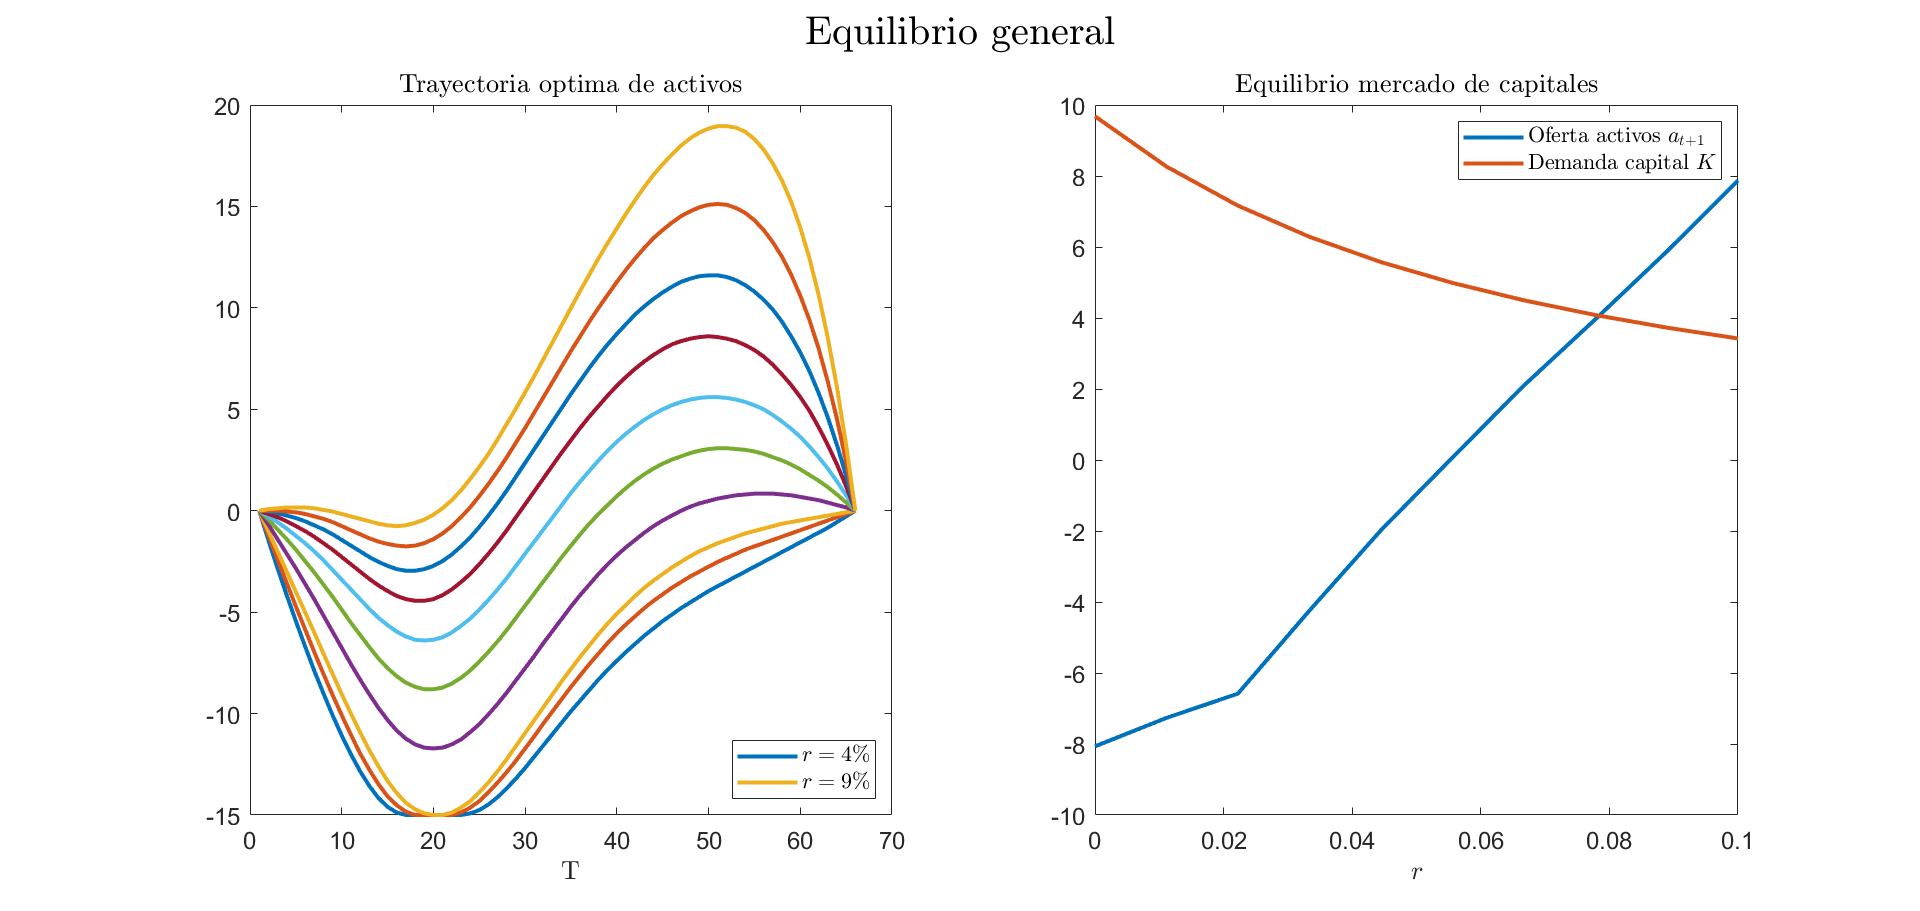
\includegraphics[width=\maxwidth{75.16307074761666em}]{figura_h}
\end{flushleft}
\end{par}

\matlabheading{i. Endogenizando $r\;y\;\omega$, encuentre la tasa de equilibrio del mercado de capitales}

\begin{par}
\begin{flushleft}
A partir del alogoritmo de bisección sobre $\frac{A-K}{K}$ encontrar la tasa de equilibrio de mercado de capitales y  explique la relación entre la \textbf{tasa de interés de equilibrio }encontrada y \textit{el gráfico desarrollado en el ítem anterior}. Además grafique la trayectoria de consumo definida por la tasa de equilibrio junto al ingreso de los agentes. Interprete económicamente. 
\end{flushleft}
\end{par}

\begin{par}
\begin{flushleft}
Para utilizar el algoritmo de bisección tenemos que tener una función objetivo a la que buscamos aproximar la solución $\rho \;\left(r\right)=0$ , en este caso $\rho \;\left(r\right)=\frac{|A-K|}{K}\;$. Además tenemos un intervalo acotado donde buscamos la solución, en este caso $r\;\epsilon \;\left\lbrack 0\ldotp 041\;0\ldotp 09\right\rbrack$ (se ha elegido el intervalo inferior dado que así permite comparar con los resultados de la pregunta anterior donde se eligió $r=\frac{1-\beta }{\beta }\approx 0\ldotp 041$. Implementaremos un número entero de 100 iteraciones, además de restringuir la solución sí y solo sí $\rho \;\left(0\ldotp 041\right)\cdot \rho \;\left(0\ldotp 09\right)<0$, pues en caso contrario no se puede asegurar la solución. Como resultado, el algortimo nos dará el punto intermedio del n-ésimo intervalo computado por el método. Además, cómo el método de bisección es una aproximación, se estimará el error $\epsilon$. 
\end{flushleft}
\end{par}

\begin{par}
\begin{flushleft}
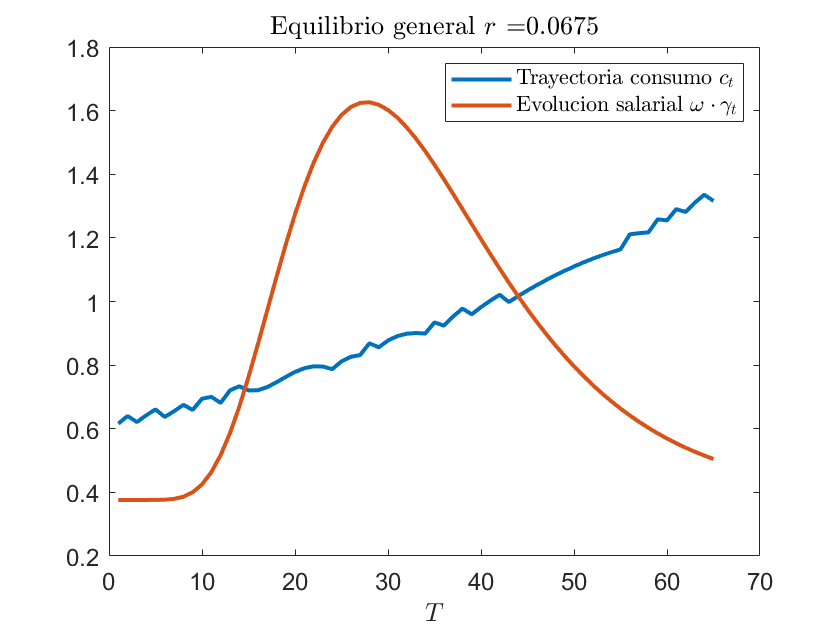
\includegraphics[width=\maxwidth{64.92724535875564em}]{figura_i}
\end{flushleft}
\end{par}

\begin{par}
\begin{flushleft}
\textit{En las siguientes preguntas, se profundizará en las implicancias de las fricciones financieras sobre el equilibrio general. Para lo anterior, defina un vector }$h{\left\lbrack 0,7\right\rbrack }_{1\textrm{x8}}$\textit{ que limita el acceso al crédito. }
\end{flushleft}
\end{par}

\matlabheading{j. Trayectoria de ciclo de vida económica}

\begin{par}
\begin{flushleft}
Grafique un subplor que muestre (1) la trayectoria de activos óptima, (2) la tasa de interés de equilibrio, (3) la trayectoria de consumo óptima (junto al ingreso) y (4) la correlación consumo-ingreso \textbf{en función de la restricción de liquidez.}
\end{flushleft}
\end{par}

\begin{par}
\begin{flushleft}
Explique la intuición económica. 
\end{flushleft}
\end{par}

\begin{par}
\begin{flushleft}
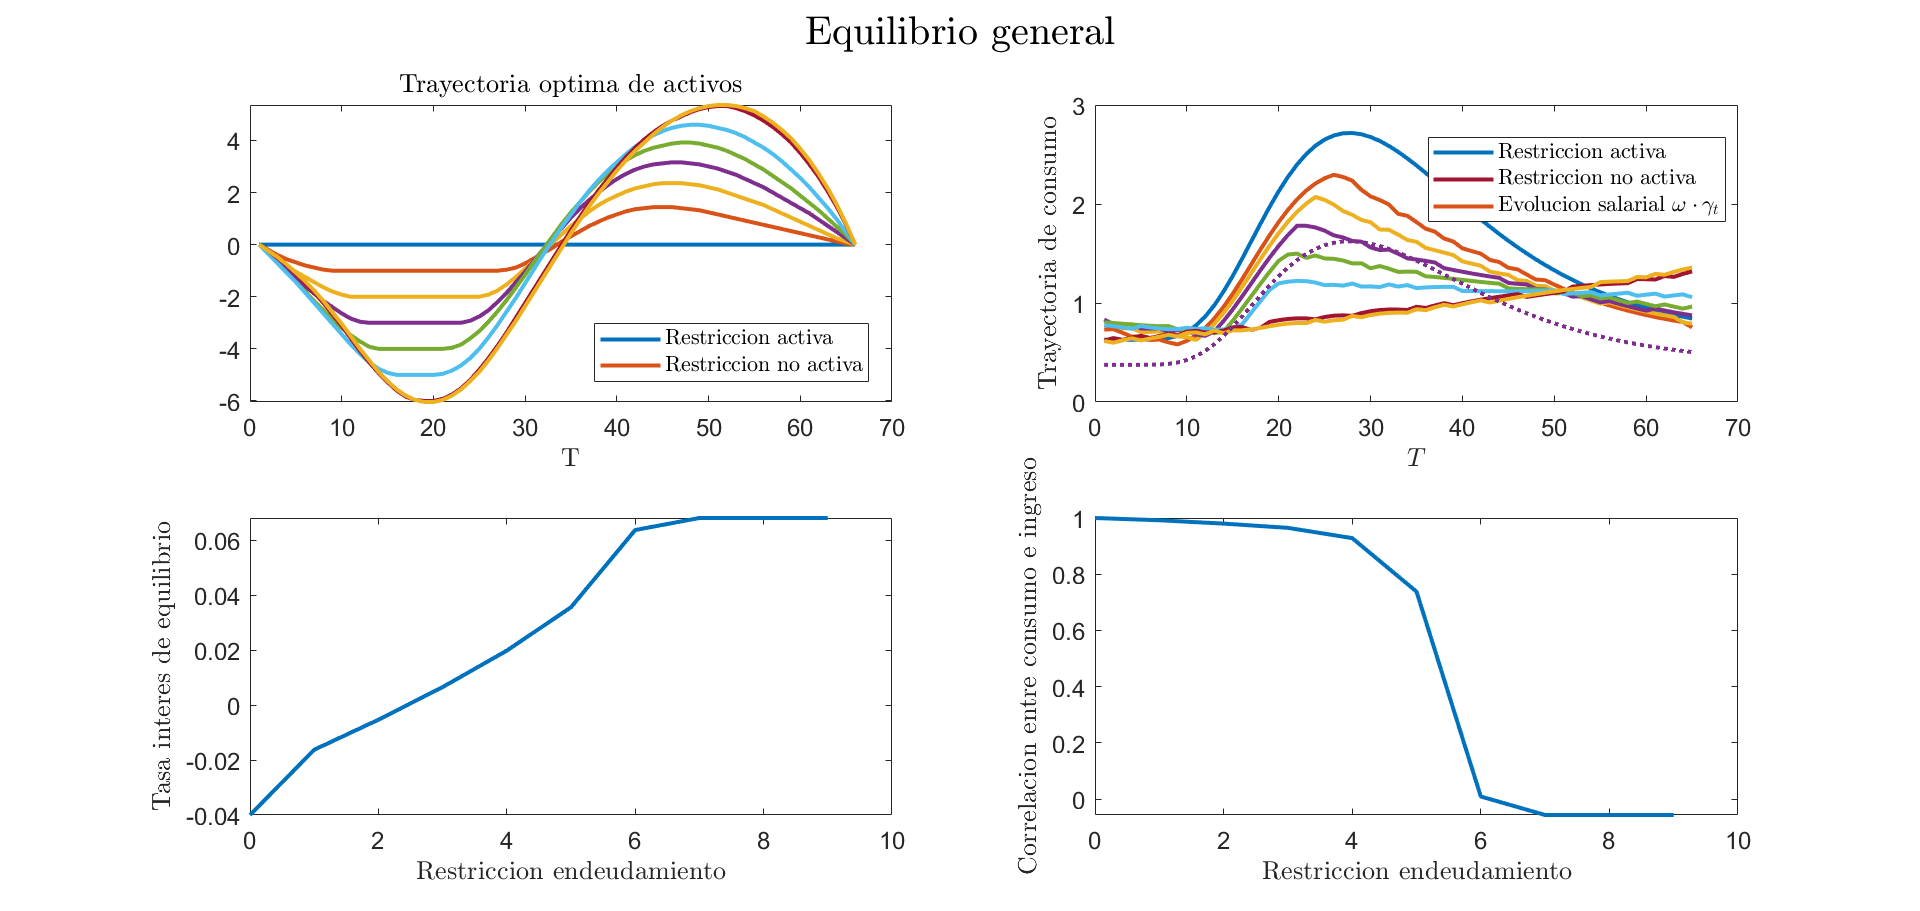
\includegraphics[width=\maxwidth{120.42147516307075em}]{figura_j}
\end{flushleft}
\end{par}

\matlabheading{k. Relación entre consumo e ingreso}

\begin{par}
\begin{flushleft}
(Ocupar Carrol)
\end{flushleft}
\end{par}

\begin{par}
\begin{flushleft}
En base a la pregunta anterior ¿Cuál es la intuición económica sobre una correlación consumo – ingreso alto cuando el acceso al crédito está muy limitado? ¿Qué sucedería con la correlación consumo - ingreso si las tasas que equilibran el mercado de capitales fueran cada vez menores? Explique conceptualmente.
\end{flushleft}
\end{par}

\end{document}
